\documentclass[10pt,a4paper]{article}

\usepackage[utf8]{inputenc}
\usepackage[english]{babel}
\usepackage[english]{isodate}
\usepackage[parfill]{parskip}
\usepackage{float}
\usepackage{graphicx}
\usepackage{float}
\graphicspath{ {./img/} }


\pagenumbering{Roman}


\title{Documentation on Scinet3}
\date{\today}
\author{Han Xiao\\ han.xiao@cs.helsinki.fi}

\begin{document}

\maketitle

\tableofcontents
\newpage

\pagenumbering{arabic}


\section{Introduction}
This documentation gives an overview of how the system works and how to use it.

\section{System workflow}

\begin{enumerate}
\item User starts by typing search query
\item Server respondes with a set of documents and keywords
\item User interacts with the app and clicks the keywords\&documents he likes. 
\item Server receives the feedback, refines the search result and return them to user. Go to step 3
\end{enumerate}

\section{Components}

Three important components are:

\begin{itemize}
\item document/keyword recommender engine, which corresponds to server side code, \verb+engine.py+
\item feedback manager that determines how feedback from documents/keywords propagate to keywords/feedback, which corresponds to browser side code, \verb+static/js/starter.js+
\item main web app that glues all above together, which corresponds to \verb+main.py+
\end{itemize}


\section{Software/library}

\begin{itemize}
\item Tornado, Python Web framework
\item MySQL, documents\&keywords data storage
\item Redis, key-value database that handles the user interaction session
\item Numpy, Python numerical library
\end{itemize}

\section{Interface}

A screencast of the Web App's interaface is  given in Figure ~\ref{fig:interface}

\begin{figure}[H]
  \centering
  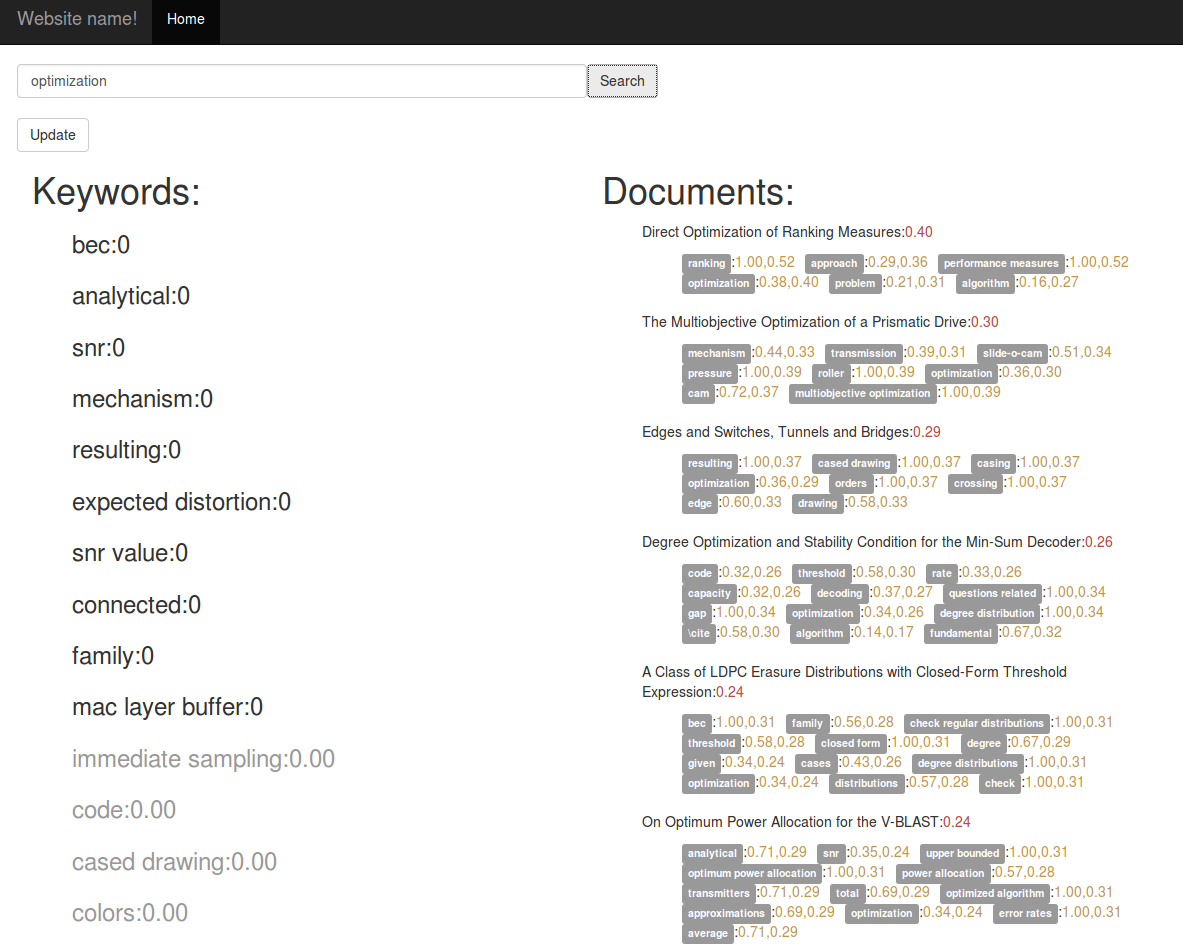
\includegraphics[scale=.25]{interface}
  \caption{Left column: the recommended keywords, in which keywords in bold are the ones being recommended while gray ones are those associated with the documents. Right column: recommended documents as well as the associated keywords}
  \label{fig:interface}
\end{figure}


\section{Running the app}
\subsection{Basic Usage}
Just go to the project directory and type:

\begin{verbatim}
python main.py [--param_name1=param_value1] [--param_name2=param_value2] ...
\end{verbatim}

If parameters are not specified, they are set on their default values.

One typical use is:

\begin{verbatim}
python main.py --table=archive_500 --recom_doc_num=10 --recom_kw_num=10 --samp_kw_num=5 \\
 --samp_doc_num=5 --linrel_doc_c=1 --linrel_kw_c=1
\end{verbatim}

Please use this one for now.

\subsection{System Parameters}

The set of parameters to control the document/keyword recommendation are:

\begin{itemize}
\item \verb+recom_kw_num+:  recommended keyword number at each iter
\item \verb+recom_doc_num+:  recommended document number at each iter
\item \verb+samp_kw_num+:  sampled keyword number from documents
\item \verb+samp_doc_num+:  extra document number apart from the recommended ones
\item \verb+linrel_kw_mu+:  Value for $\mu$ in the linrel algorithm for keyword
\item \verb+linrel_kw_c+:  Value for $c$ in the linrel algorithm for keyword
\item \verb+linrel_doc_mu+: Value for $\mu$ in the linrel algorithm for document
\item \verb+linrel_doc_c+:  Value for $c$ in the linrel algorithm for document
\end{itemize}

Basic system setup parameters are:

\begin{itemize}
\item \verb+port+:  the given port  the web app runs on
\item \verb+mysql_port+:  database's port 
\item \verb+mysql_host+: database host
\item \verb+mysql_user+:  database user
\item \verb+mysql_password+:   database password
\item \verb+mysql_databas+:  database name
\item \verb+redis_port+:  redis' port 
\item \verb+redis_host+: key-value cache host
\item \verb+redis_db+: key-value db
\item \verb+table+:  document table table to be used 
\item \verb+refresh_pickle+: refresh pickle, which saves the precomputed feature matrices, or no
\end{itemize}

\section{Feedback}

Feedbacks are allowed to propagate, which means user can indirectly give feedbacks to keywords when they interacts with the documents and vice versa.

\subsection{Rule of Thumb}

Let's define:
\begin{enumerate}
  \item explicit feedback: the feedback user gives to either the keyword or the document by clicking. For example, if the user clicks keyword Python, Python receives feedback 1
  \item implicit feedback: the feedback received through feedback propagation. For example, if user clicks some document, then the keywords associated with the document receives some implicit feedback.
  \item final feedback: which consists of the explicit feeedback and implicit one and it is the actual feedback value for the LinRel algorithm.
\end{enumerate}

Rule of thumb on feedback propagation is:
if the keyword/document has receives some explicit feedback, any implicit feedback to it will not contribute to the final feedback. 
Otherwise, the final feedback value will only consider the implicit part.

The intuition of this design is: if the user is quite sure/explicit about the preference over something, any guessing(implicit) is not necessary. Implicit guessing is only used when there is not enough information.

\subsection{Calculation}

Explicit feedback is discrete can only be 1 or 0. It is 1, if the object is clicked and 0 otherwise.

Implicit feedback is continuous, from 0 to 1.

Using keyword to illustrate how implicit feedback calculation is done. If $kw_i$ is associted with $doc_1 \cdots doc_k$(they contain $kw_i$), the implicit feedback value for $kw_i$ is:

\begin{equation}
fb_{implicit}(kw_i) = \sum\limits_j{tfidf(doc_j, kw_i) \cdot I(doc_j, kw_i)}
\end{equation}

where:
\begin{enumerate}
\item $I(doc_j, kw_i)$ is an indicator function giving 1 if $kw_i$ in $doc_j$ is clicked and 0 otherwise
\item $tfidf(doc_j, kw_i)$ is the TfIdf value of $doc_j$ on $kw_i$
\end{enumerate}

Implicit feedback calculation on document is the same, except using the tf-idf value of keyword on document.


\section{Keyword\&document recommendation}

\subsection{Query-based recommender}

This is used as initial starting point of the app when user searches by inputing some query. See QueryBasedRecommender in engine.py for the actual code.

The process goes like this:
\begin{enumerate}
\item select the \verb+recom_doc_num+ docs by ranking them by the similarity scores to the query. 
\item sample \verb+recom_kw_num+ keywords from docs in Step 1.
\item sample \verb+samp_kw_num+ keywords from any docs that share any keywords with the docs in Step 1(to diversify the recommended keywords).
\item sample \verb+samp_doc_num+ docs from docs that contain any keywords from Step 3(to diversify the recommended documents).
\end{enumerate}

\subsection{LinRel-based recommender}

This is the recommender engine using LinRel algorithm as its core. See LinRelRecommender in engine.py for the actual code.

\subsubsection{Document recommendation}
\label{linrel-doc-recom}

Using:
\begin{enumerate}
\item $y_t$: formed by document feedback history
\item $D_t$: formed by document that have received feedbacks
\item $D$: document to keyword TdIdf matrix 
\end{enumerate}
to calculate the scores for each document and return the top \verb+recom_doc_num+ to the user.


\subsubsection{Keyword recommendation}

Similar things happen to the keywords recommendation:

Using:
\begin{enumerate}
\item $y_t$: formed by keyword feedback history
\item $D_t$: formed by keyword that have received feedbacks
\item $D$: keyword to keyword TdIdf matrix 
\end{enumerate}

to calculate the scores for each document and return the top \verb+recom_kw_num+ to the user.

To allow for richer feedback information, keywords associated with the recommended documents in section ~\ref{linrel-doc-recom} is also returned to the user(but displayed in a less obvious way)

\section{Sampling methods}
Sampling methods are applied during the LinRel-based documents\&keywords recommendation. The purposes are:
\begin{enumerate}
\item to reduce the matrix dimension involved in the LinRel algorithm so as to speed up the process
\item add randomness to document\&keyword selection in order to ``explore out''
\end{enumerate}

Thus, the recommendation process changes from:

\begin{enumerate}
\item receive feedback from user
\item using the LinRel to rank the documents\&keywords
\item return the top N documents\&keywords to the user
\end{enumerate}

to:

\begin{enumerate}
\item receive feedback from user
\item sample a subset of documents\&keywords for LinRel to rank(for dimension reduction)
\item using the LinRel to rank the sampled documents\&keywords
\item sampling a subset of documents\&keywords(for exploring out)
\item return the top N documents\&keywords from the sampled set to the user
\end{enumerate}

The following subsections are organized by the two different purposes of sampling.

\subsection{Dimension reduction}
This sampling process prepares the set of documents\&keywords for LinRel computation and it is performed in the following way:

\begin{enumerate}
\item sample documents, $docs_{sampled}$: sample from the set of documents, $docs_{source}$, which satisfy \textit{any} of the following: 
  \begin{enumerate}
  \item it has received some feedback \footnote{This point is mentioned by our last meeting}
  \item any of its keywords has feedback\footnote{This point is mentioned by our last meeting}
  \item it is similar to any of the documents with feedback received \footnote{The purpose of this step is to further add some exploration}
  \item it contains keywords that are similar to the keywords with feedback received\footnote{Same purpose as the above point}
  \end{enumerate}
\item sample keywords, $kws_{sampled}$: sample from the set of keywords, $kws_{source}$ which satisfy \textit{any} of the following: 
  \begin{enumerate}
  \item it has received some feedback\footnote{This point is mentioned by our last meeting}
  \item any of its documents has feedback\footnote{This point is mentioned by our last meeting}
  \item it is similar to any of the keywords with feedback received\footnote{Same purpose as the above point}
  \item it is associated with documents that are similar to documents with feedback received\footnote{Same purpose as the above point}
  \item it is associated with any documents appearing in $docs_{source}$ or $docs_{sampled}$ \footnote{In order to let the returned documents and keywords be more assocaited with each other}
  \end{enumerate}
\end{enumerate}


We can reverse the above sampling order, starting from keyword sampling first, and do the sampling in a similar fashion.

\subsection{Exploring out}
An extra sampling can be applied to the ranked documents\&keywords produced by LinRel algorithm in order to further ``explore out''.

But I don't think this extra sampling is necessary because the purpose of ``exploring out'' for both documents and keywords are already done by LinRel algorithm. Adding a extra layer of sampling might not do any good, even it might decrease the result quality.

\section{Source code}

Source code is managed using git at \verb+https://vcs.hiit.fi/git/scinet3+.


\newpage 

\listoffigures
\newpage
\listoftables
\newpage

\end{document}
